\section{Osrank}
\label{s:osrank}

\def\Graph{\mathsf{Graph}}
\def\proj{\mathsf{project}}
\def\contributor{\mathsf{account}}
\def\dep{\mathsf{depend}}
\def\own{\mathsf{maintain}}
\def\coown{\mathsf{maintain}^\circ}
\def\contrib{\mathsf{contrib}}
\def\cocontrib{\mathsf{contrib}^\circ}

\oscoin{}的基础机制之一是将区块奖励的一部分分发给网络内的高质量项目,所以\oscoin{}协议必须对哪些项目质量高达成一致。为了选出收到\oscoin{}奖励的项目并决定其奖励份额,\oscoin{}网络使用\osrank{}算法对项目之间的关系图和其对网络的贡献进行评价。\osrank{}是著名的\pagerank{}算法的变种,其输出形式是给每个项目$P$一个对应的分数$\omega(P)$。

\subsection{出发点}

虽然判断一个开源软件包的重要性是高度主观的行为,但是通过研究开源软件的依赖关系和贡献结构,能够得到一个项目相对重要程度很有价值的信息。

与Google围绕分析网页超文本结构的\pagerank{}算法开发出的大规模搜索引擎类似,开源软件依赖与贡献关系的图结构也能对表示其在生态中被信任程度和相对价值提供重要的依据。

\subsection{原理}

一个系统作为整体产生的价值可能十分明了,但是特定子系统贡献的价值往往并不清晰。而且不同的子系统将价值转换成收益的能力本质上就有所不同。那些位于与其他域相邻的边界位置的子系统往往在这个方面更有优势,尽管它们产生的价值可能更多汲取自其他子系统。这种子系统价值流输入输出的不平衡对系统整体不利。

幸好人类活动并不发生在虚空之中:无论是脑力劳动、内容创作、金融活动等等,实体之间有意义的互动都被每个实体拥有的相对于系统整体而言的相对价值深深影响。重要的一点是,在活动的过程中产生了一系列的人类活动产物(超媒体链接、合同、转账、依赖关系等等),这些痕迹是不同实体之间关系具象的证明。

由\pagerank{}以及类似的度量方式带给我们的一个基本思考是,通过对系统内代理人有意义活动痕迹的近似模拟,产生与观察相符的成系列的人类活动产物,我们就可以研究子系统中的价值流动,进而估算内含的价值分布。就\pagerank{}而言,其模拟的是人类在互联网上搜索相关度高的数据,得到的是一系列链接。一个高级的算法在选择下一个链接的时候会使用尽可能多的启发式的方法(正如人类行为那样),比如,衡量链接文本的相关性。如果计算资源稀缺,粗糙的算法会简单地随机选择下一条链接。这就是产生经典的\pagerank{}公式的原因。该方法已经在互联网上被证明十分成功。

\subsection{标记符号}

在这一部分,我们将使用如下表示方法:图指有限有向图。对于图$G$,顶点的集合表示为$V(G)$,边的集合表示为$E(G) \subseteq V^2$。$G$的一条边$e = (x,y)$表示为$x \xrightarrow[]{e} y$。对于一个给定的G顶点的子集X,$G[X]$表示X的诱导子图,即以X为顶点集、以$\{ x \xrightarrow[]{e} y \mid e \in E(G), \{x,y\} \subseteq X\}$为边集的图。图$G$内一次长度为n的途径是图的态射$L_n \to G$,$L_n$是第$n$个线性图:$V(L_n) = \{i \in \mathbb{N} \mid i \leq n \}$,
$E(L_n) = \{ (i,i+1) \in \mathbb{N}^2 \mid i < n \}$。

\subsection{\Oscoin{}里的排序实体}
\label{s:netgraph}

被\oscoin{}账本捕捉到的与OSS开发相关的人类活动产物有:
\begin{itemize}
  \item 项目的维护,
  \item 项目之间的依赖关系,
  \item 项目内经过签名的代码贡献。
\end{itemize}
我们将这些交互总结为一个带权有向图$G$。权重反映相应边的相对重要性,并设置为算法的超参数。以一个顶点为起点的所有边的权重之和为$1$。

\begin{center}
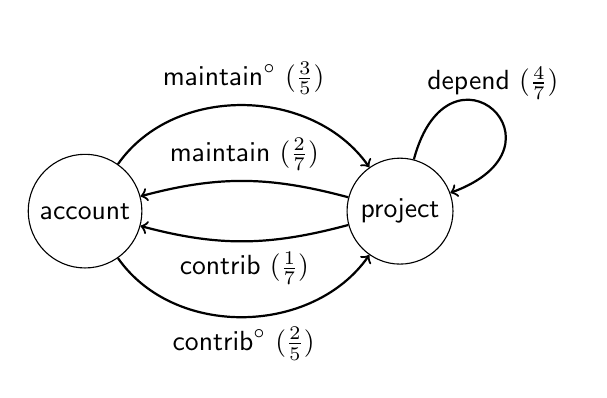
\begin{tikzpicture}[vertex/.style={draw,circle,minimum width=8ex}, arr/.style={draw,thick,->}]
  \node[vertex] (p) at (2,0)  {\Small $\proj$};
  \node[vertex] (u) at (-2,0) {\Small $\contributor$};

  \draw[arr,looseness=7] (p) to[out=75,in=20] node[above] {\Small $\dep \ (\frac{4}{7})$} (p);
  \draw[arr] (p) to[out=165,in=15] node[above]   {\Small $\own \ (\frac{2}{7})$} (u);
  \draw[arr] (u) to[out=55,in=125] node[above]   {\Small $\coown \ (\frac{3}{5})$} (p);
  \draw[arr] (p) to[out=195,in=-15] node[below]  {\Small $\contrib \ (\frac{1}{7})$} (u);
  \draw[arr] (u) to[out=-55,in=-125] node[below] {\Small $\cocontrib \ (\frac{2}{5})$} (p);
\end{tikzpicture}
\captionof{figure}{\small 开源软件开发中实体关系的图解(权重仅为示例)\label{fig:G}}
\end{center}
\medskip

% TODO: include simulations description and results here.

\noindent 值得注意的是,某些关系会是双向的,但每个方向的权重并不一定相同。例如,$\contrib$和〖$\cocontrib$∘从属于同一个人类活动产物:一个账户对一个项目的代码贡献。$\contrib$边表示的命题为:对于项目而言,贡献者有价值。反向的$\cocontrib$∘边表示的命题为:项目对于贡献者来说是有价值的。对于这个不太明显的反向流动的解释是,开发者往往不会在他们觉得没有用的项目上贡献时间。

% TODO: Make the above easier to grasp. Also maybe rephrase a little "is
% valueable to the project"

虽然依赖关系图是一个项目从另一个项目汲取价值最直接的指示,但添加对应贡献和维护的边仍然能够服务于两个目的:
\begin{itemize}
\item 依赖关系图是有向的:方向从用户端应用指向核心库。这会将分数极大地向基础库和开发工具倾斜。将贡献包括进去将带来反向的流动,标识出有价值的用户端应用。例如,一个功能全面的开源文本编辑器对于开源开发者来说十分有价值,但是它可能永远不会在另一个软件明确的依赖关系中出现。但是,向这个文本编辑器贡献代码的开发者也有可能向这个编辑器使用的包贡献代码。这将使得算法从代码库向用户端包反向流动价值。
\item 仅仅依靠依赖关系无法充分地将不同域连接起来。开发者经常向相邻的生态贡献代码和工具,使原本独立的项目能够有所联系。这样,一个将依赖关系和代码贡献结合起来的图可能会充分地联系起来,揭示开源项目潜在的价值。
\end{itemize}
我们提议将这些人类活动产物(依赖关系、代码贡献等)记录为区块链的转账。这样,就可以在$G$之上可验证地构建一个能够达成共识的有限有向图$\netgraph$(即在图$\Graph/G$的一个切片范畴内),用来表示\oscoin{}网络图。

反过来,这使得全局价值分数能够依据模拟随机漫步的特定随机过程分配给实体,即$\netgraph$内的活动轨迹结合从$G$得到的取样概率。例如,一个贡献者决定在一个高价值的项目上进行开发,贡献一个变动。贡献者在这个过程中将另一个项目加入了依赖关系。这个依赖关系引入了一个来自上游包的错误。因此这个贡献者转换方向来解决这个存在在路径中的错误,以此类推。这个过程很像人类点击链接搜索信息过程的模拟。这个模拟活动告诉了我们在广泛的OSS生态系统中子系统之间的价值流动。

这个我们称为\osrank{}的分数被用来将判断项目对\oscoin{}网络的价值,并将区块奖励的一部分分发给项目。

\subsection{定义}

为了实现\osrank{},我们采用如下蒙特卡洛类算法:对于网络内的每个顶点,都将开始$R$个随机漫步。在选择下一顶点时,首先会由取样的边基于$G$内的权重选择边的类型。下一步行动会由边的类型决定:

\begin{itemize}
\item 对于依赖与维护边,所有顶点的可能性相同。
\item 对于从贡献者$x$指向项目$p$的边$x \xrightarrow[]{\coown} p$,项目$p$被选择的概率是$\frac{p_x}{N_x}$ 。$p_x$是$x$贡献给p的数量,$N_x$是$x$贡献的总数。
\item   对于$p \xrightarrow[]{\contrib} x$边,贡献者x被选中的概率为$\frac{p_x}{N}$。$N$是$p$从所有贡献者处收到的贡献的总数。
\end{itemize}

\noindent 对于每一步,漫步在项目顶点处结束的概率是$1 - \epsilon_\proj$,在账号顶点则为$1 - \epsilon_\contributor$ (这里的$\epsilon_\proj, \epsilon_\contributor \in (0,1)$是阻尼因子)。这就产生了$nR$个随机漫步的集合$W$。$n$是顶点的总数。一个项目$x$的\osrank{}为:
\[
  \omega(x) = \frac{W_x (1-\epsilon_\proj)}{n R}
\]
$W_x$是$W$内经过$x$的漫步的次数,即:
\[
  W_x = \sum_{w \in W} |w[\{x\}]|.
\]
相似地,账户$a$的\osrank{}为:
\[
  \omega(a) = \frac{W_a (1-\epsilon_\contributor)}{n R}.
\]

\subsection{女巫攻击}

为了维持\oscoin{}网络图的完整性,非法的生态系统必须被剔除。这意味着以利用\osrank{}为目的发起的欺骗性的项目与贡献结构必须被算法惩罚。这种针对PageRank的女巫攻击已经在之前被细致地研究过。

为了解决这个问题,我们以TrustRank~\cite{trustrank}的逻辑为基础,提出了对\pagerank{}算法的修改。这包括两个阶段:

\begin{itemize}
\item   在第一阶段,所有的随机漫步开始于起始种子集合$\seedset$内的一个顶点。Υ是为了这个目的而从所有项目和账户顶点中选出的一个子集。这样得到的分数会偏向与种子集合的交互,但是这些分数不会直接被奖励机制使用。这个过程是为了得到一个阈值$t$,进而确定实体的合法性:任何分数低于阈值的实体都不会继续进行下一阶段。这一阶段的输出是网络图的一个子图$\netgraph_t$。
\item 在第二阶段,将会在子图$\netgraph_t$上以同样的方式运行算法,只不过不再使用种子集合。第二阶段输出的结果为\osrank{}。
\end{itemize}
在选择种子集合的时候必须十分小心,以确保其足够大并且足够分散,使得从这些顶点开始的随机漫步能够能够触及到网络内所有的合法项目。维持这样一个种子集合有很多方式。这个部分将在今后进行更深入的探讨。

\subsection{信息可靠性与\osrank{}}

实施\osrank{}时需要考虑的一个重要因素是账本上信息的可靠性,即,依赖关系。这是网络图N实质化的基础。

为了使\osrank{}成为在网络内价值的良好代表,账本上的信息必须准确。虽然提出的算法能够允许一定程度的误差,但我们也必须依靠大部分所声明的关于依赖关系与贡献的事实的准确与及时。按事实情况来说,项目与维护者存在固有的社会层面的动机来及时更新依赖信息,也就是说,依赖信息对每个人都是公开可见的,项目也需要在依赖者间维持自己的声誉。此外,项目存在着被分叉的风险,而\osrank{}又与经济激励有关,所以对于项目来说,来自自己周身生态环境的信任就显得很重要。

然而,从长期来看,这些激励可能不足以阻止不诚实方从这个系统中取得不正当利益。我们将在第七章中简要讨论可能的解决方案。\S\ref{s:future-work}

\subsection{实施}

为了确保\osrank{}的计算不会变得过分昂贵,以至于运营者无法进行计算,系统使用了以下几个方法。

\begin{itemize}
\item 增量蒙特卡洛。为了使\osrank{}值能在网络图改变时及时更新,我们使用了增量算法。这个算法依赖的基础事实是在两次计算之间,只增加或减少了少量顶点或边,所以无需每次从零计算\osrank{}。因此,大多数在之前计算中实施的随机漫步在更新后的图中仍然有效。例如,如果从上次计算至今只增加了$p_1 \xrightarrow[]{\dep} p_2$一个依赖关系,那么只有在上次计算过程中经过$p_1$的随机漫步才会失效。

    在实际运行过程中,网络的运营者会将上次计算的随机漫步集合存储在缓存内,并及时在更新时删除无效漫步,加入新的漫步。关于增量\pagerank{}算法的细节请见*。\cite{incr pagerank}

    由于所有计算必须是确定性的,这些漫步并不是真随机。这些随机漫步的启动必须借助一个内置的伪随机数产生器\footnote{在无需许可设定中设计一个适当的随机数生成器是一个正在被活跃地研究的领域。现存解决方案存在近期的文献中有所描述,这部分内容超出了本文的范围。}。

\item 长周期。在这个场景下,根据\osrank{}做出的支付被控制得频率很低。这就必须将奖励周期值设定得很大,比如,每月一次。这种情况下,滥用者可能在奖励发放区块之前修改数个项目的网络结构。为了缓解这个问题,边的权重会考虑其在上个周期内的寿命。例如,如果一个依赖关系在奖励区块之前$n$个区块被添加,那么它的权重比例就只有$n/\epoch$。\end{itemize}

\bigskip

\noindent 正如\S \ref{s:treasury}解释的那样,在账本上存储\osrank{}是\oscoin{}的货币政策的基础。而且,\osrank{}与$\netgraph$将会可以被智能合约调用,项目能够使用这是数据定制特性。